\chapter{Экспериментальный раздел}

\section{Исследование появления блокировок}

Основной задачей исследования сетей Петри является выявление недоступных состояний и блокировок. Выявим причины, по которым они могут возникнуть в диаграммах деятельности. В процессе исследования представим диаграмму деятельности в виде простой и раскрашенной сети Петри и сравним результаты.

В диаграммах деятельности блокировки могут возникать по причине:
\begin{itemize}
\item неверной структуры диаграммы;
\item невозможности перехода из-за невыполнения логического условия спусковой функции.
\end{itemize}

\subsection{Простая сеть Петри}

Так как простые сети Петри могут моделировать лишь поток выполнения, для них возможно выявления лишь структурных несоответствий диаграммы.

Блокировки в сетях Петри могут быть вызваны лишь ситуацией, когда переходу принадлежит два и более места, но не все места имеют фишки. Применительно к диаграмме деятельности, только блок ожидания завершения параллельного процесса может иметь больше одной входной дуги во внутреннем переходе. Таким образом, для получения блокировки внутри блоков многопоточной обработки должен находиться условный переход (рис. \ref{fig:fig22}, \ref{fig:fig23}).

\begin{figure}
	\begin{minipage}[H]{0.49\linewidth}
		\center{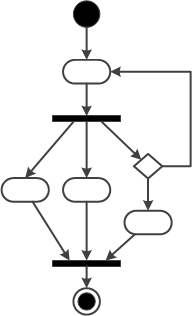
\includegraphics[scale=1]{include/BlockedDiagram1.png}}
	\end{minipage}
	\hfill
	\begin{minipage}[H]{0.49\linewidth}
		\center{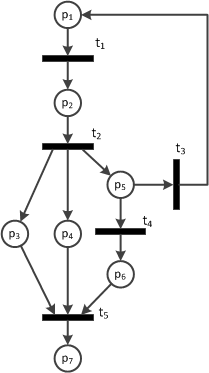
\includegraphics[scale=1]{include/BlockedNet1.png}}
	\end{minipage}
	\caption{Блокировка из-за выхода за пределы блоков.}
	\label{fig:fig22}
\end{figure}

\begin{figure}
	\begin{minipage}[H]{0.49\linewidth}
		\center{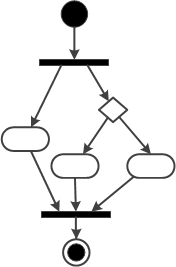
\includegraphics[scale=1]{include/BlockedDiagram2.png}}
	\end{minipage}
	\hfill
	\begin{minipage}[H]{0.49\linewidth}
		\center{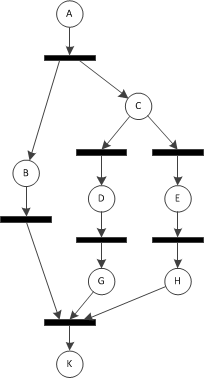
\includegraphics[scale=1]{include/BlockedNet2.png}}
	\end{minipage}
	\caption{Блокировка из-за неверной структуры внутреннего условия.}	
	\label{fig:fig23}	
\end{figure}

Ситуация блокировки, изображенная на рисунке \ref{fig:fig22} искусственная, т.к. по логике выход за пределы параллельных процессов невозможен. Так же, при моделировании такой ситуации получается, что метки C и D являются небезопасными, и в них будет происходить бесконечное накопление фишек.

Ситуация, изображенная на рисунке \ref{fig:fig23} возможна и в результате в системе возникает блокировка, т.к. переход никогда не сработает. Для избежания такой ситуации используется введение дополнительной вершины, из которой будет единственная дуга в блок синхронизации (рис. \ref{fig:fig24}).

\begin{figure}
	\begin{minipage}[H]{0.49\linewidth}
		\center{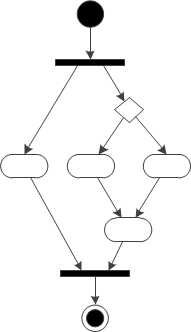
\includegraphics[scale=1]{include/CorrectDiagram.png}}
	\end{minipage}
	\hfill
	\begin{minipage}[H]{0.49\linewidth}
		\center{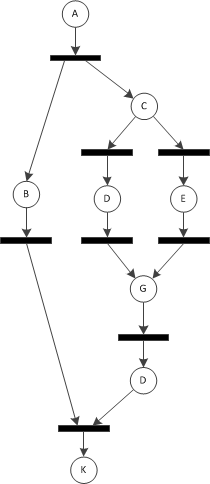
\includegraphics[scale=1]{include/CorrectNet.png}}
	\end{minipage}
	\caption{Корректная структура внутреннего условия.}	
	\label{fig:fig24}	
\end{figure}

\subsection{Раскрашенная сеть Петри}

Диаграмма деятельности имеет практически линейную структуру, за исключением вершины условного перехода, которая при преобразовании в простую сеть будет давать два возможных пути выполнения, т.к. переходы имеют равный приоритет и в простой сети срабатывание перехода определяется лишь наличием фишки в позиции. При наличии некоторого цикла в диаграмме, анализ с помощью простой сети Петри выдаст лишь его наличие.

Моделирование работы диаграммы деятельности с помощью раскрашенных сетей Петри приводит к тому, что пути процесса выполнения будут иметь вид линейную структуру, а не древовидную. Блокировка в сети может быть вызвана не только отсутствием фишки в позиции, но и не срабатыванием спусковой функции из-за невыполнения логического условия.

По этой причине, раскрашенная сеть Петри не всегда способна выявить некорректную структуру диаграммы, т.к. при конкретной начальной разметке, для которой построена сеть, не все переходы будут активны.

\section{Исследование корректности построения раскраски сети}

Предложенный метод формирования раскраски сети на основе определения максимальной видимости переменных в ходе исследования работоспособности метода дал хорошие результаты, но при этом были выявлены ограничения, связанные со структурой преобразуемой диаграммы.

Если в диаграмме имеется хотя бы один цикл, то при наложении раскраски возникает вопрос об определении области видимости переменных. В связи с этим получается два подхода:
\begin{itemize}
\item[1.] определять раскраску всех элементов цикла как кортеж переменных наибольшей мощности (рис. \ref{fig:fig25});
\item[2.] определять раскраску не учитывая обратную дугу цикла (рис. \ref{fig:fig26}).
\end{itemize}

Так как фишка хранит в себе набор переменных, сопоставленных ее цвету, то при реализации первого подхода на переходах внутри цикла будут меняться лишь значение переменных. Такой подход будет вести к некорректному моделированию работы, т.к. если какая либо позиция в цикле содержит несколько фишек, то в процессе моделирования будет использована лишь одна из них, и весь процесс работы будет привязан лишь к значениям переменных.

При реализации второго подхода в сети может случиться блокировка, т.к. фишка из раскраски меньшей мощности будет переходить к более мощной раскраске в позиции не содержащей фишек новой раскраски. Другими словами, при моделировании работы диаграммы на рисунке \ref{fig:fig26} не сможет сработать переход $ t_{6} $ даже если будет выполнено логическое условие, ограничивающее этот переход, т.к. мощность раскраски позиции $ p_{6} $, содержащей фишку, меньше мощности позиции $ p_{2} $.

\begin{figure}
	\begin{minipage}[H]{0.49\linewidth}
		\center{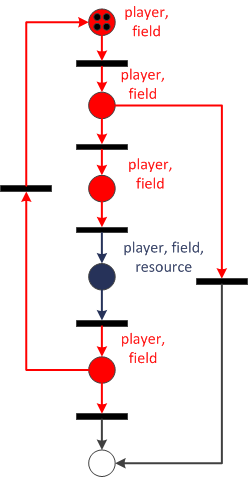
\includegraphics[scale=1]{include/ResearchWithCycle.png}}
		\caption{Сеть с раскраской, наложенной с учетом циклов.}
		\label{fig:fig25}
	\end{minipage}
	\hfill
	\begin{minipage}[H]{0.49\linewidth}
		\center{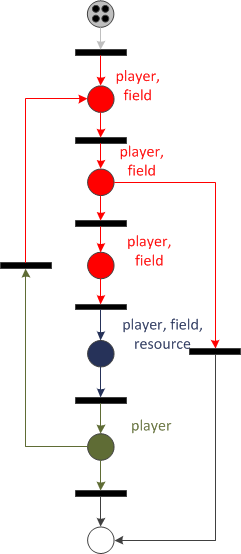
\includegraphics[scale=1]{include/ResearchWithoutCycle.png}}
		\caption{Сеть с наложением раскраски без учета циклов.}
		\label{fig:fig26}
	\end{minipage}
\end{figure}

С учетом вышесказанного было принято решение использовать первый подход, но при нахождении в позиции с ненулевой разметкой заменять фишку, содержащуюся в маркере на новую. Это решение позволяет избежать некорректности работы модели, т.к. в процессе будут использоваться все фишки сети.

\section{Сравнение скорости работы простой и раскрашенной сети Петри}

Проведем сравнение времени работы и затраченных ресурсов для моделирование работы диаграммы деятельности, представленной простой и раскрашенной сетью Петри.

В сравнении времени моделирования учитывалось только время преобразования диаграммы деятельности в сеть и проведение анализа. Результаты сравнения показаны в \ref{tab:table1}.

\begin{table}
	\caption{Сравнение времени моделирования.}
	\begin{tabular}{|l|c|c|c|}
	\hline
	& 8 состояний & 15 состояний & 25 состояний \\
	\hline
	Простая сеть Петри & 0.012 сек. & 0.015 сек. &  0.020 сек. \\
	\hline
	Раскрашенная сеть Петри & 0.42 сек. & 0.67 сек. &  0.114 сек. \\
	\hline
	\end{tabular}
	\label{tab:table1}
\end{table}

В результате исследования мы получили, что время, затраченное для моделирования раскрашенной сеть Петри значительно больше. Это объясняется тем, что на этапе преобразования диаграммы помимо самого преобразования в сеть Петри происходит так же анализ множества используемых переменных и построение раскраски. Так же во время моделирования для раскрашенной сети на каждом переходе происходит вычисление новых значений переменных, а для каждой дуги из позиции в переход вычисляется спусковая функция.

Для подсчета затраченных ресурсов использовался профилировщик кода VTune. Профилировщик запускал моделирующую программу и по окончанию моделирования выводился список затраченных ресурсов для каждого объекта программы.

\begin{table}
	\caption{Сравнение затраченных ресурсов.}
	\begin{tabular}{|l|c|c|c|}
	\hline
	& 8 состояний & 15 состояний & 25 состояний \\
	\hline
	Простая сеть Петри & 250KB & 340KB & 585KB \\
	\hline
	Раскрашенная сеть Петри & 345KB & 420KB & 730KB \\
	\hline
	\end{tabular}
	\label{tab:table2}
\end{table}

В результате исследования было выявлено, что моделирование диаграммы деятельности в виде простой и раскрашенной сети Пери требует приблизительно одинаковое количество ресурсов. Небольшая разница объясняется тем, что в раскрашенной сети для каждой позиции хранится список используемых переменных и цвет, а в переходах и на внутренних дугах содержится выражения.

\label{cha:research}

